\chapter{基于马尔科夫过程的模式文本匹配}

由于文本匹配的适用领域较为广泛,因此在各大互联网公司得到了大量的应用,创造了巨大的商业价值。基于强化学习的文本匹配可以较好的建模模式匹配中的规则。本文介绍了强化学习的主要技术,并且提出了模式文本匹配的算法设计。

\section{马尔科夫决策过程}
强化学习中,在某一时刻 $t$ ,主体会处于状态 $s_t$,并从环境中得到观测 $o_t$,根据观测和行动利用策略 $\pi_\theta(a_t|o_t)$ 或者 $\pi_\theta(a_t|s_t)$作出行动 $a_t$,环境根据主体状态 $s_t$ 以及行动 $a_t$ 通过转移概率分布函数 $p(s_{t+1}| s_t, a_t)$ 得到状态 $s_{t+1}$,通过奖励函数 $r(s, a)$ 得到奖励 $r_t$,周而复始。强化学习的目标即最大化总收益。

\begin{figure}[!htbp]
    \centering
    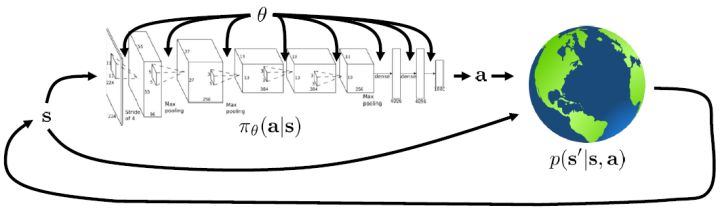
\includegraphics[width=1.0\textwidth]{MDP}
    \bicaption{马尔科夫决策过程}{Markov Decision Process}
    \label{fig:MDP}
\end{figure}

状态 $s$,行动 $a$,奖励函数 $r(s,a)$ 以及转移概率 $p(s'|s,a)$ 定义了马尔科夫决策过程。

在描述马尔科夫决策过程前,先简要介绍马尔科夫链。马尔科夫链 $M=\{S, P\}$ 由状态空间 $S$ 和转移概率 $P$ 组成。其中状态 $s$既可以是离散的变量,也可以是连续的数值;转移概率$p(s_{t+1}|s_t)$ 确定了在当前状态下转移到下一个状态的概率。令转移概率 $P_{i, j}=p(s_{t+1}=i|s_t=j)$,则这些概率组成了概率转移矩阵 $\mathcal{P}$。马尔科夫链具有马尔科夫性,即转移概率只与当前的状态有关。

马尔科夫过程是马尔科夫链在决策环境中的扩展 $M=\{S, A, P, R, \pi\}$。其中状态空间 $S$ 与马尔科夫链类似;行动空间 $A$ 即行动的集合;转移概率 $P$ 不仅受到当前状态的影响,还受到行动 $a\in A$ 的影响;$R$ 为奖励函数,是一个 $S\times A\to \mathbb{R}$ 的映射;策略 $\pi$ 表示在当前状态下每个行为的概率。

强化学习的过程中 $S, A, P, R$ 都是环境确定的,我们需要学习 $\pi(a|s)$ 以最大化长期收益。$\pi(a|s)$  可以由一个参数为 $\theta$ 的模型确定,记为 $\pi_\theta(a|s)$。

考虑一个有限长度的轨迹 $\tau=\{s_1,a_1,...s_t,a_t\}$,它产生的概率
$$
p_\theta(\tau) = p(s_1)\prod_{t=1}^T \pi_\theta(a_t|s_t)p(s_{t+1}|s_t,a_t)
$$
初始状态 $s_1$ 往往是确定的。根据马尔科夫性,后面每个时刻的行动和状态都是由当前的行动确定的。我们希望优化
$$\theta^* = \arg\max_\theta E_{\tau\sim p_\theta(\tau)}[\sum_t r(s_t, a_t)]$$以最大化总收益函数关于轨迹的期望。

对于有限长度的轨迹,我们在求解 $\theta^*$ 时只需要关注马尔科夫链在一个时间点上的边际分布;对于无限长度的轨迹,根据马尔科夫性,有
$$\left[\begin{array}{l}\mathbf{s}_{t+k}\\\mathbf{a}_{t+k}\end{array}\right]=\mathcal{P}\left[\begin{array}{l}\mathbf{s}_{t+k-1}\\\mathbf{a}_{t+k-1}\end{array}\right]=...=\mathcal{P}^k\left[\begin{array}{l}\mathbf{s}_{t}\\\mathbf{a}_{t}\end{array}\right]$$
对于无限长度的问题,当到达平稳分布时,我们可以对目标进行平均:
$$
\theta^*=\arg\max_\theta\frac{1}{T}\sum_{t=1}^T\mathbf{E}_{(\mathbf{s}_t,\mathbf{a}_t)\sim p_\theta(\mathbf{s}_t,\mathbf{a}_t)}r(\mathbf{s}_t,\mathbf{a}_t)\rightarrow \mathbf{E}_{(\mathbf{s},\mathbf{a})\sim p_\theta(\mathbf{s},\mathbf{a})}r(\mathbf{s},\mathbf{a})
$$

一个完整的强化学习的训练过程一般包含 3 个部分:

1. 生成样本。在模拟器中运行我们当前的策略并收集轨迹(trajectory)样本。轨迹的收集即主体和环境的交互过程:在 $t$ 时刻,我们从环境得到观测信息 $o_t$,在此观测信息下根据策略 $\pi_\theta(a_t|o_t)$ 得到当前的行动 $a_t$,根据系统的转移概率 $p(s_{t+1}|s_t, a_t)$ 得到下一个状态 $s_{t+1}$。在做出当前的行动之后,我们会得到收益 $r(s_t,a_t)$, 简记为 $r_t$ 。我们的目标就是最大化得到的总收益。

2. 收益估计。不同的算法在这一步的表现不尽相同。对于策略学习来说,就是策略评估;对于基于模型的增强学习算法,就是模型拟合。

3. 改进策略。根据上一步得到的结果改进策略,再执行第一步,循环往复。

\begin{figure}[!htbp]
    \centering
    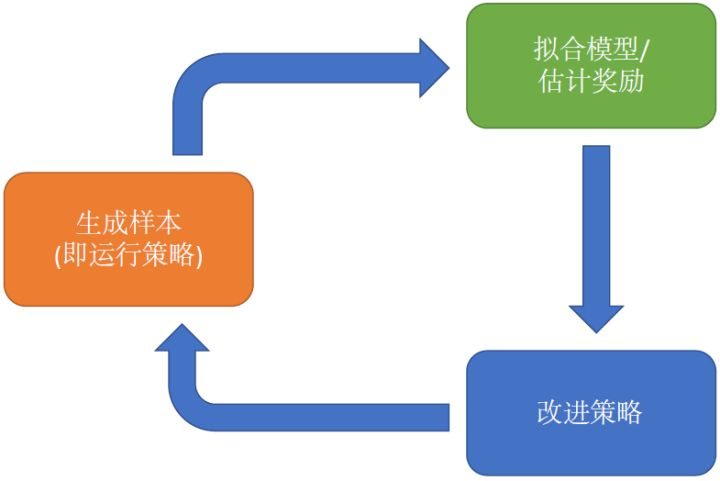
\includegraphics[width=0.5\textwidth]{RL_process}
    \bicaption{增强学习算法的一般步骤}{Reinforcement Learning Process}
    \label{fig:RL_process}
\end{figure}

\subsection{马尔科夫决策过程求解}

但是由于强化学习中在样本生成时得到的行动以及系统的状态转移都带有一定的随机性,因此我们希望最大化奖励的条件期望
\begin{equation}\label{eq:max_expect}
G_t = R_{t+1} + \gamma R_{t+2} + ... = \sum_{k=0}^\infty \gamma^kR_{t+k+1}
\end{equation}
$\gamma$ 表示折现率。

我们将值函数(value fuction)定义为一个状态在未来的价值,即回报的期望。那么值函数可以被表示为:
\begin{equation}\label{eq:Bellman}
\begin{aligned}
v(s) & = E[G_t|S_t = s] \\
     & = E[R_{t+1} + \gamma R_{t+2} + \gamma^2 R_{t+3}+...|S_t=s]\\
     & = E[R_{t+1} + \gamma(R_{t+2} + \gamma R_{t+3}+...)|S_t=s]\\
     & = E[R_{t+1} + \gamma G_{t+1}|S_t=s]\\
     & = E[R_{t+1} + \gamma v(S_{t+1})|S_t=s]\\
\end{aligned}
\end{equation}

\eqref{eq:Bellman} 被称为 Bellman 方程,它表明 value function 可以通过迭代计算得到。我们的目的就是通过迭代优化最大化 $v(s)$

通过 Bellman 方程,我们可以得到:
\begin{equation}
\begin{aligned}
v_{k+1}(s) & = E[R_{t+1} + \gamma v_k(S_{t+1})|S_t=s]\\
           & = \sum_a \pi(a|s)\sum_{s',r}p(s', r| s, a)[r+\gamma v_k(s')]
\end{aligned}
\end{equation}
我们可以通过迭代计算价值函数来优化策略收敛到最优。

策略迭代一般分成两步:策略评估和策略改进。利用当前策略产生新样本,使用新样本更新当前策略,最终收敛到最优。在策略评估时需要知道环境的状态转移概率,因此策略迭代需要依赖模型。

\begin{algorithm}[H]
    \small
    \caption{policy iteration}\label{alg:policy_iteration}
    \begin{algorithmic}
        \State Step 1. Initialization
        \State $V(s) \in \mathbb{R}$ and $\pi(s) \in \mathcal{A}(s)$ aribitrarily for all $s \in \mathcal{S}$
        \State Step 2. Policy Evaluation
        \Repeat
        \State $\Delta \leftarrow 0$
        \For {each $s \in \mathcal{S}$}
        \State $v \leftarrow V(s)$
        \State $V(s)\leftarrow \sum_{s', r} p(s', r|s, \pi(s))[r + \gamma V(s')]$
        \State $\Delta \leftarrow \max(\Delta, |v-V(s)|$
        \EndFor

        \Until{$\Delta < \theta$}

        \State Step 3. Policy Improvement
        \State policy-stable $\leftarrow  true$
        \For {each $s \in \mathcal{S}$}
        \State $a \leftarrow \pi(s)$
        \State $\pi(s) \leftarrow \arg\max_a\sum_{s', r}p(s', r|s, \pi(s))[r + \gamma V(s')]$
        \State If $a \neq \pi(s)$ then policy-stable $\leftarrow  false$
        \EndFor
        \State If policy-stable, then stop and return V and $\pi$; else go to 2
    \end{algorithmic}
\end{algorithm}

但是策略迭代算法每次都要进行策略评估和改进,这大大增加了算法的训练时间。由于对策略的改进和对值函数的改进是一致的,所以我们可以将策略改进视为对值函数的改进。

通过 Bellman 方程,我们可以得到:
\begin{equation}\label{eq:Bellman_value}
\begin{aligned}
v_{*}(s) & = E[R_{t+1} + \gamma v_*(S_{t+1})|S_t=s, A_t=a]\\
         & = \max_a \sum_{s',r}p(s', r| s, a)[r+\gamma v_k(s')]
\end{aligned}
\end{equation}

从 \eqref{eq:Bellman_value} 可以发现,我们可以通过 Bellman 最优模型来更新值函数收敛,最后收敛可以得到当前策略的最优值 $v_*$

\begin{algorithm}[!htbp]
    \small
    \caption{value iteration}\label{alg:value_iteration}
    \begin{algorithmic}
        \State Initialization array $V$ aribitrarily
        \Repeat
        \State $\Delta \leftarrow 0$
        \For {each $s \in \mathcal{S}$}
        \State $v \leftarrow V(s)$
        \State $V(s)\leftarrow \max_a\sum_{s', r} p(s', r|s, a)[r + \gamma V(s')]$
        \State $\Delta \leftarrow max(\Delta, |v-V(s)|$
        \EndFor
        \Until{$\Delta < \theta$}

        \State Output a deterministic policy, $\pi$ such that
        \State $\pi(s) = \arg\max_a\sum_{s', r} p(s', r|s, a)[r + \gamma V(s')]$
    \end{algorithmic}
\end{algorithm}

相比于 \ref{alg:policy_iteration},值迭代算法避免了策略评估部分的计算量,降低了算法运行时间,有效地提高了算法的运行效率。

我们发现无论是算法 \ref{alg:policy_iteration} 还是 \ref{alg:value_iteration},算法每次都是选择概率或者是值最高的行动。这种策略被称为利用(exploitation)。与之相对应的,如果我们每次都根据概率或者是值的分布进行采样,根据采样的结果采取行动,这种策略被称为探索(exploration)。探索的优势在于当信息匮乏是可以取得较好的效果,但是效率很低;利用的优势在于效率很高,但是只有在信息足够充足的情况下才会有效。

将探索和利用结合的算法被称为 $\epsilon$-贪心算法。我们在每次选择行动的时候,都以 $\epsilon$ 的概率进行探索,以 $1-\epsilon$ 的结果进行利用好。可以通过 $\epsilon$ 的调整在算法的不同阶段达到不同的效果。

\section{文本匹配的MDP介绍}
\label{sec:TM_MDP}
本节将文本匹配过程建模为一个强化学习过程。

在模式文本匹配的过程中,我们可以将文本匹配的过程与编辑距离\citep{website:edit_dis}的计算过程类比。coffee 和 cafe 的编辑距离计算过程可以被表示为

\begin{figure}[H]
    \centering
    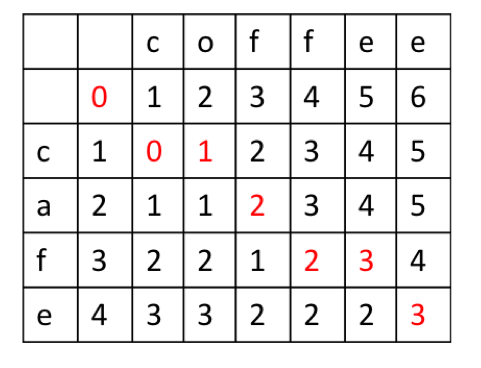
\includegraphics[width=0.40\textwidth]{LD_dis}
    \bicaption{编辑距离计算过程}{Edit distance}
    \label{fig:LD_dis}
\end{figure}

图\ref{fig:LD_dis}红色的部分为编辑距离的匹配路径。我们也可以将文本匹配表示为类似的过程:

\begin{figure}[!htbp]
    \centering
    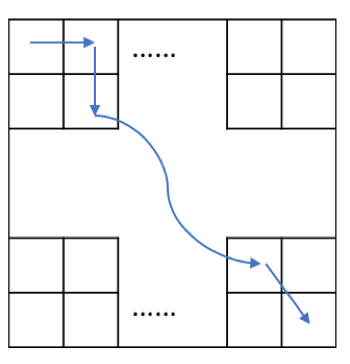
\includegraphics[width=0.40\textwidth]{match_MDP}
    \bicaption{模式文本匹配计算过程}{Pattern Text Matching}
    \label{fig:match_MDP}
\end{figure}

和 MatchPyramid 以及 MatchSRNN 类似,我们同样会使用匹配矩阵的概念。我们从匹配矩阵的右上角出发,根据当前位置确定行走方向,直到走到左下角为止。这样情况下我们会得到一条匹配路径。我们需要建立一个判别模型,根据匹配路径判断是否匹配。

首先描述文本匹配算法中获得匹配路径的过程,该过程为一个马尔科夫决策过程。

我们将文本匹配的状态表示为在匹配矩阵中的位置 $s_t = [q_{t}, d_{t}]$,其中 $q_{t}, d_{t}$ 分别表示$t$时刻在第1,2个句子中的位置。
和编辑距离类似,文本匹配的过程中也有3种行为:向下走,向右走和向右下方走。
在$t$时刻,我们根据系统的状态 $s_t$ 得到当前的观测 $o_t = Q [q_{t}:k+q_{t}], D [d_{t}:k+d_{t}]$,即从当前位置开始,将两个句子的前 $k$ 个单词作为输入,并通过值函数获得每个行动的值。式中 $Q, D$ 分别表示2个句子。

\begin{figure}[!htbp]
    \centering
    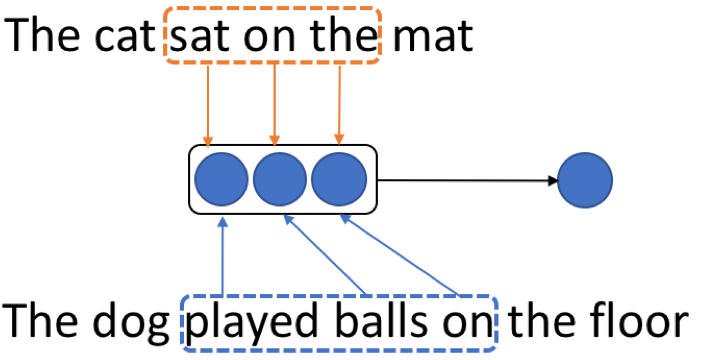
\includegraphics[width=0.40\textwidth]{match_value_function}
    \bicaption{文本匹配值函数输入}{value function input of text matching}
    \label{fig:value_function_input}
\end{figure}

值函数以两个句子当前位置的前 $m$ 个单词作为输入,确定当前句子是否可以正确判别。
我们利用一个 LSTM 网络处理输入的序列,通过对 LSTM 网络输出的加权和进行线性变换得到值函数:
$$
V(s) = \sigma(<w, g(s)>, b_v)
$$

其中 $g(s)$ 是LSTM网络的输出:

$$
g(s) = LSTM(Q[q_{t}:m+q_{t}], D [d_{t}:m+d_{t}])
$$

LSTM 网络接受两个长度为 $m$ 的单词序列,计算得到隐状态:

\begin{equation}
\label{eq:LSTM}
\begin{aligned}
f_k &= \sigma(W_f[Q_{k+q_{t}}, D_{k+d_{t}}] + U_fh_{k-1} + b_f) \\
i_k &= \sigma(W_i[Q_{k+q_{t}}, D_{k+d_{t}}] + U_ih_{k-1} + b_i) \\
o_k &= \sigma(W_o[Q_{k+q_{t}}, D_{k+d_{t}}] + U_oh_{k-1} + b_o) \\
c_k &= f_k \circ c_{K-1} + i_k \circ (W_c[Q_{k+q_{t}}, D_{k+d_{t}}] + U_ch_{k-1}+b_c) \\
h_k &= o_k \circ \text{tanh}(c_k)
\end{aligned}
\end{equation}

图 \ref{fig:value_function_input} 以 $Q=\{\text{The cat sat on the mat}\},D=\{\text{The dog played balls on the floor}\}, m=3$ 为例展示了值函数。当前的状态 $s=[2, 2]$ ,我们将 $Q[2:5]=\{\text{sat, on, the}\}, D[2:5]=\{\text{played, balls, on}\}$ 的词向量作为 LSTM 的输入,利用 LSTM 捕捉未来词汇的序列信息,计算每个行为的值。

环境的状态转移都是确定性的,即
\begin{equation}
\label{eq:status_transfer}
S_{t+1} =
\begin{cases}
[q_{t} + 1, d_{t}], & \quad{\rm walk\,down} \\
[q_{t}, d_{t} + 1], & \quad{\rm walk\,right} \\
[q_{t} + 1, d_{t}+1], & \quad{\rm walk\,lower\,right}
\end{cases}
\end{equation}
环境的奖励为模型是否可以预测成功,即 $\mathbf{1}_{t=y}$,其中 $t$ 为预测的 label, $y$ 为实际label。

获得匹配路径的算法可以被表示为:
\begin{algorithm}[!htbp]
    \small
    \caption{MDP of Text Match}\label{alg:MDP_TM}
    \renewcommand{\algorithmicrequire}{\textbf{Input:}}
    \renewcommand{\algorithmicensure}{\textbf{Output:}}
    \begin{algorithmic}
        \Require Labeled data $D=\{ (\mathbf{Q}, \mathbf{D}, \mathbf{Y}) \}$
        \Ensure Path
        \State \text{Initialize} Path $\leftarrow [0, 0]$
        \State {set $q_1=0, d_2=0$}
        \While {$q_t < \text{len}(\mathbf{s}_1)$ and $d_t < \text{len}(\mathbf{s}_2)$}
        \State $a_t = \arg\max_a v(Q [q_t:m+q_t], D [d_t:m+d_t], a)$
        \State update status according to Eq \ref{eq:status_transfer}
        \State Path $\leftarrow$ Path $\oplus [q_t, d_t]$ \Comment{$\oplus$ means appends to end}
        \EndWhile
    \end{algorithmic}
\end{algorithm}

在计算路径时,算法从初始状态 $s_1 = [Q[1:m], D[1:m]]$ 出发,每次将当前位置的前 $k$ 个词作为输入,得到每个行动的值,选择值最大的行动作为当前的行动,并根据当前的行为移动到下一个位置,直到到达矩阵的右下角。一直选择值最大的行动可能会导致算法陷入局部最优解,因此可以采用 $\epsilon$-贪心的方法控制探索和利用的程度。

\subsection{匹配路径的判别}
\label{sec:path_classify}

在计算匹配路径之后,我们需要根据路径判断两个句子是否匹配。判别算法以原句子 $Q, D$ 以及对应的路径映射 $m_1 = [q_1, q_2, \cdots, q_t], m_2 = [d_1, d_2, \cdots, d_t]$ 作为输入,判断两个句子是否匹配。

我们利用3个LSTM网络作为判别模型,其中 LSTM$_1$ 和 LSTM$_2$ 将 $S_1$ 和 $S_2$ 映射为2个矩阵,LSTM$_c$ 将这两个矩阵映射为一个一维向量 $g_c(s)$:
$$
\begin{aligned}
f(Q) &= \text{LSTM}_1(Q) \\
h(D) &= \text{LSTM}_2(D) \\
g_c(s) &= \text{LSTM}_c([{f(Q)}_{q_1}, {h(D)}_{d_1}], [{f(Q)}_{q_2}, {h(D)}_{d_2}], \cdots, [{f(Q)}_{q_t}, {h(D)}_{d_t}])
\end{aligned}
$$

通过对 $g_c(s)$ 的加权和进行归一化得到最终的匹配概率
$$
p = \sigma(<w, g_c(s)> + b)
$$
其中 $w$ 和 $b$ 都是需要学习的参数,$\sigma(x) = \frac{1}{1+e^{-x}}$
LSTM 网络和 \ref{eq:LSTM} 类似, LSTM$_1$  和 LSTM$_2$ 共享参数。

\begin{figure}[!htbp]
    \centering
    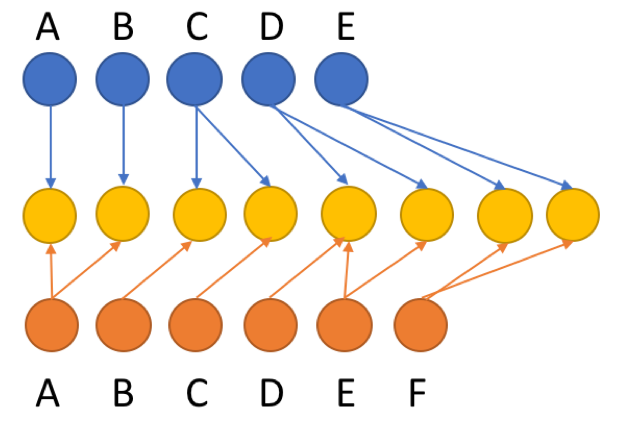
\includegraphics[width=0.40\textwidth]{path_classify}
    \bicaption{匹配路径判定}{match path classfiy}
    \label{fig:path_classify}
\end{figure}

\section{文本匹配 MDP 的训练与预测}
上节引入了文本匹配的 MDP,本节主要介绍文本匹配的MDP的训练与预测过程。
\subsection{训练过程}
训练时我们使用算法 \ref{alg:value_iteration} 进行优化。模型的参数包含 MDP 过程的参数 $\Theta_{MDP}$ 以及判别模型的参数 $\Theta_{c}$,在训练时,模型接受数据集 $D=\{Q^{(n)}, D^{(n)}, Y^{(n)}\}_{n=1}^N$ 作为输入,输出参数 $\Theta_{MDP}$ 以及 $\Theta_{c}$.

在训练阶段,每次迭代时,利用算法 \ref{alg:MDP_TM} 为每个样本$Q, D$生成一条路径

$$\{[q_1, d_1], [q_2, d_2], \cdots, [q_t, d_t]\}$$

并根据生成的路径以及真实结果训练路径判别模型。训练路径匹配模型时的损失函数为交叉熵:
\begin{equation}
\label{eq:classify_model}
\ell_c(Y, p) = -(Y\log(p) + (1-Y)\log(1-p))
\end{equation}

在路径判别模型收敛后,利用判别模型输出该路径为匹配的概率 $p$, 并利用 $p$ 计算奖励:
$$
r = \log(\frac{1}{|p-Y+\Delta|})
$$
其中 $\Delta$ 表示一个极小值以保证 $|p-Y+\Delta| > 0$.

之后我们利用$r$更新 $\Theta_{MDP}$。 MDP 过程的损失函数为:
\begin{equation}
\label{eq:MDP_model}
\ell(V(s), r) = \sum_{i=1}^t\left((y - V(r_i))^2\right)
\end{equation}

\begin{algorithm}[!htbp]
    \small
    \caption{Train Process of Text Match}\label{alg:TM_train}
    \renewcommand{\algorithmicrequire}{\textbf{Input:}}
    \renewcommand{\algorithmicensure}{\textbf{Output:}}
    \begin{algorithmic}
        \Require Labeled data $D=\{ (\mathbf{Q}^{(n)}, \mathbf{D}^{(n)}, \mathbf{Y}^{(n)})\}_{n=1}^N$, learning rate $\eta$
        \Ensure $\Theta_{MDP}, \Theta_{c}$
        \State \text{Initialize} $\Theta_{MDP}, \Theta_{c} \leftarrow$ random values in $[-1, 1]$
        \While {not convergency}
          \State generate path according to Alg~\ref{alg:MDP_TM}
          \While {not convergency}
            \State $\Theta_{c} = \Theta_{c} - \eta \frac{\delta \ell_c}{\delta \Theta_{c}}$ \Comment{$\ell_c$ is defined in Eq~\ref{eq:classify_model}}
          \EndWhile
          \State $\Theta_{MDP} = \Theta_{MDP} - \eta \frac{\delta \ell}{\delta \Theta_{MDP}}$ \Comment{$\ell$ is defined in Eq~\ref{eq:MDP_model}}
        \EndWhile
    \end{algorithmic}
\end{algorithm}

\section{实验与结果分析}
\subsection{实验数据}
为了对我们提出的文本匹配 MDP 的有效性进行评估,我们利用 Quora 的问题匹配数据集进行了测试。 Quora 是美国的在线知识问答平台,每天会产生大量的相似问题。该数据集即为 Quora 从其问答平台上收集到并进行了人工标注的匹配问题数据。

该数据集共包含约40万数据集,句子长度从3到100不等,能够较好的对模型的有效性进行评估。由于该数据集的样本量过大,我们从样本中挑选出了长度在 8到10 的约6万个句子对作为数据集,选择其中的 45056 个句子对作为训练集,22528个句子对作为验证集,4441个句子作为测试集对我们的算法进行了测试。

\subsection{评价准则}
为了比较不同算法的预测结果,本小节介绍用于文本匹配算法的评价准则。对于测试集 $S = \{S_1^{(n)}, S_2^{(n)}, Y^{(n)}\}_{n=1}^N$,文本采用的评价准则如下所述:

\begin{itemize}
  \item[•] 准确率: 计算<句子对,标签> 被正确划分的次数占总样本的比重。 $\text{acc}(S)$ 越大,算法在该准则上的表现越好;当 $\text{acc}(S) = 1$ 时,该评价指标达到最优值。
  $$
  \text{acc}(S) = \frac{\sum_i^N\mathbb{I}_{y_i=t_i}}{N}
  $$
  其中 $y_i$ 表示第 $i$ 个样本的预测结果, $t_i$ 表示第 $i$ 个样本的实际结果。
  \item[•] F1:对 <句子对,标签> 正样本准确率以及负样本准确率的调和平均值。 $\text{F1}(S)$ 越大,算法在该准则上的表现越好;当 $\text{F1}(S) = 1$ 时,该评价指标达到最优值。
  $$
  \begin{aligned}
  \text{P}(S) &= \frac{\sum_i^N\mathbb{I}_{y_i=t_i \text{and} t_i = 1}}{\sum_i^N\mathbb{I}_{t_i = 1}}\\
  \text{R}(S) &= \frac{\sum_i^N\mathbb{I}_{y_i=t_i \text{and} t_i = 0}}{\sum_i^N\mathbb{I}_{t_i = 0}}\\
  \text{F1}(S) &= \frac{2*P*R}{P+R}
  \end{aligned}
  $$
  \item[•] auc:ROC(Receiver Operating Characteristic) 曲线和坐标轴相交部分覆盖的面积大小。 ROC 曲线由两个变量 1-specificity 和 Sensitivity 绘制,分别反映了负样本和正样本的分类准确率。$\text{auc}(S)$ 越大,算法在该准则上的表现越好;当 $\text{auc}(S) = 1$ 时,该评价指标达到最优值。
\end{itemize}

\subsection{实验结果}
\label{sec:lab_value}
对于文本匹配问题,目前已经有多种算法可以很好地解决该问题。本文选取了其中两个经典的文本匹配算法 MatchPyramid\ref{Pang2016TextMA} 以及 MatchSRNN\ref{Wan2016MatchSRNNMT} 来与本文提出的算法进行比较。

在 Quora 数据集上。本文进行了算法的五折交叉验证。即将原始数据集合分割成五份,每份大小相同。每一折实验选择其中的四份数据作为训练集,一份数据作为验证集。上述过程重复五次,即每份数据都被用做验证集。每一折实验都选取验证集上评价准则最高的参数进行测试,将测试结果取平均值作为最后的评估结果。

\begin{table}[!htbp]
    \bicaption{文本匹配算法在 Quora 数据集上的测试结果}{The result of text matching algorithm on Quora dataset}
    \label{tab:MDP_test}
    \centering
    \footnotesize% fontsize
    \setlength{\tabcolsep}{4pt}% column separation
    \renewcommand{\arraystretch}{1.2}%row space
    \begin{tabular}{cccc}
        \hline
        \multirow{2}{*}{Algorithm} &
        \multicolumn{3}{c}{\multirow{1}{*}{Evaluation Criterion}} \\
        \cline{2-4} & acc & F1 & auc \\
        \hline
        Matching MDP & $\textbf{0.7222}(*)$ & $0.7217$ & $\textbf{0.7979}(*)$ \\
        MatchPyramid & $0.7130$ & $\textbf{0.7220}(*)$ & $0.7853$ \\
        MatchSRNN & $0.7105$ & $0.7201$ & $0.7848$\\
        \hline
    \end{tabular}
\end{table}

可以发现 Matching MDP 的方法在 acc 和 auc 上均显著优于 MatchPyramid 和 MatchSRNN, 在 F1 上三者相差并不大。

但是由于 value iteration 基于贪心的策略导致算法很容易陷入过拟合,因此我们在Quora数据集上选取了10240个句子对进行测试。测试方法同样采用五折交叉验证:

\begin{table}[H]
    \bicaption{文本匹配算法在 Quora 小数据集上的测试结果}{The result of text matching algorithm on small Quora dataset}
    \label{tab:MDP_small_test}
    \centering
    \footnotesize% fontsize
    \setlength{\tabcolsep}{4pt}% column separation
    \renewcommand{\arraystretch}{1.2}%row space
    \begin{tabular}{cccc}
        \hline
        \multirow{2}{*}{Algorithm} &
        \multicolumn{3}{c}{\multirow{1}{*}{Evaluation Criterion}} \\
        \cline{2-4} & acc & F1 & auc \\
        \hline
        Matching MDP with $\epsilon$ = 0 & $0.6465$ & $0.6644$ & $0.7056$ \\
        Matching MDP with $\epsilon$ = 0.1 & $0.6519$ & $\textbf{0.6772}(*)$ & $0.7080$ \\
        Matching MDP with changed $\epsilon$ & $0.6532$ & $0.6612$ & $0.7147$ \\
        \hline
        MatchPyramid & $\textbf{0.6671}(*)$ & $0.6702$ & $0.7237$ \\
        \hline
        MatchSRNN & $0.6617$ & $0.6736$ & $\textbf{0.7285}(*)$\\
        \hline
    \end{tabular}
\end{table}

从表格 \ref{tab:MDP_small_test} 可以发现,在小数据集下 Matching MDP 算法出现了明显的过拟合,人工调节的 $\epsilon$ 可以小幅度提高算法的效果,但是仍然无法超过 MatchPyramid 和 MatchSRNN。

\subsection{本章小结}
本章主要介绍了文本匹配的马尔科夫决策过程。首先介绍了马尔科夫决策过程的背景,包括马尔科夫链以及马尔科夫决策过程的训练和推断,并且根据文本匹配的场景对文本匹配的MDP进行了形式化描述,并利用值迭代的方法进行训练和推断。该模型在大数据量的情况下表现优异,但是由于值迭代算法的缺陷,在小数据场景下表现不佳。在后续章节中,本文将针对该问题进行改进。
